%%*****************************************************************************
%% $Id: history.tex 7056 2008-05-17 18:36:00Z gene $
%%*****************************************************************************
%% Author: Gerd Neugebauer
%%-----------------------------------------------------------------------------
\documentclass[11pt,a4paper]{scrartcl}

\usepackage[latin1]{inputenc}
\usepackage{tikz}
\providecommand\BibTeX{\textsc{Bib}\TeX}

\begin{document}%%%%%%%%%%%%%%%%%%%%%%%%%%%%%%%%%%%%%%%%%%%%%%%%%%%%%%%%%%%%%%%

\BibTeX~0.98i
\BibTeX~0.99b Feb 1988
\BibTeX~0.98c

\BibTeX~8 1996

ML\BibTeX 2001
ML\BibTeX 1.3 2003

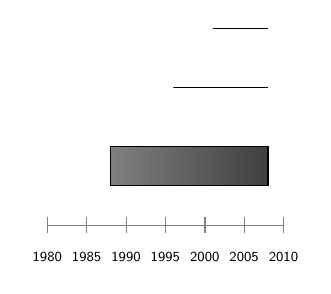
\begin{tikzpicture}\tiny\sf
  \draw[gray,thin] (198.0,-0.5) -- (201.0,-0.5);

  \draw[gray,thin] (198.0,-0.4) -- (198.0,-0.6);
  \draw (198.0,-.9) node{1980};
  \draw[gray,thin] (198.5,-0.4) -- (198.5,-0.6);
  \draw (198.5,-.9) node{1985};
  \draw[gray,thin] (199.0,-0.4) -- (199.0,-0.6);
  \draw (199.0,-.9) node{1990};
  \draw[gray,thin] (199.5,-0.4) -- (199.5,-0.6);
  \draw (199.5,-.9) node{1995};
  \draw[gray,thin] (200.0,-0.4) -- (200.0,-0.6);
  \draw (200.,-.9) node{2000};
  \draw[gray,thin] (200.5,-0.4) -- (200.5,-0.6);
  \draw (200.5,-.9) node{2005};
  \draw[gray,thin] (201.0,-0.4) -- (201.0,-0.6);
  \draw (201.,-.9) node{2010};

  \shadedraw[left color=gray, right color=gray!50!black] (198.8,.5) rectangle (200.8,0);
  \shadedraw[left color=gray, right color=gray!50!black] (199.6,1.25) rectangle (200.8,1.25);
  \shadedraw[left color=gray, right color=gray!50!black] (200.1,2) rectangle (200.8,2);
\end{tikzpicture}

\end{document}%%%%%%%%%%%%%%%%%%%%%%%%%%%%%%%%%%%%%%%%%%%%%%%%%%%%%%%%%%%%%%%%%
%
% Local Variables: 
% mode: latex
% TeX-master: nil
% End: 
